\documentclass[
    reprint,
    amsmath,amssymb,
    aps,
    pra,
    superscriptaddress,
    floatfix
]{revtex4-2}

\usepackage{graphicx}
\usepackage{dcolumn}
\usepackage{bm}
\usepackage{mathtools}
\usepackage{braket}
\usepackage{tikz}
\usetikzlibrary{arrows.meta,positioning,calc,decorations.pathmorphing}
\usepackage{quantikz}
\usepackage{hyperref}
\usepackage{amsthm}

% APS-style theorem formatting
\newtheoremstyle{aps}%
  {}{}%
  {}%
  {\parindent}%
  {\itshape}%
  {.}%
  { }%
  {}%

\theoremstyle{aps}
\newtheorem{theorem}{Theorem}
\newtheorem{lemma}{Lemma}
\newtheorem{example}[theorem]{Example}

% Custom commands
\newcommand{\C}{\mathbb{C}}
\newcommand{\R}{\mathbb{R}}
\newcommand{\N}{\mathbb{N}}
\newcommand{\Z}{\mathbb{Z}}
\newcommand{\T}{\mathbb{T}}
\newcommand{\Sphere}{\mathbb{S}^2}
\newcommand{\CP}{\mathbb{C}\mathrm{P}^1}
\newcommand{\SU}{\mathrm{SU}}
\newcommand{\SO}{\mathrm{SO}}
\newcommand{\U}{\mathrm{U}}
\newcommand{\Tr}{\mathrm{Tr}}
\newcommand{\re}{\mathrm{Re}}
\newcommand{\im}{\mathrm{Im}}

\newcommand{\PauliI}{\sigma_0}
\newcommand{\PauliX}{\sigma_x}
\newcommand{\PauliY}{\sigma_y}
\newcommand{\PauliZ}{\sigma_z}

\newcommand{\rtilde}{\tilde{r}}
\newcommand{\TB}{\mathrm{TB}}
\newcommand{\SB}{\mathrm{SB}}

\begin{document}

\title{Quantum state preparation on the real line with stereographic quantum signal processing}

\thanks{This manuscript has been authored by UT-Battelle, LLC, under Contract No.\ DE-AC05-00OR22725 with the U.S.\ Department of Energy (DOE). The United States Government retains and the publisher, by accepting the article for publication, acknowledges that the United States Government retains a non-exclusive, paid-up, irrevocable, world-wide license to publish or reproduce the published form of this manuscript, or allow others to do so, for United States Government purposes. The Department of Energy will provide public access to these results of federally sponsored research in accordance with the DOE Public Access Plan.}

\author{Tyler Kharazi}
\affiliation{Department of Chemistry, University of California, Berkeley, California 94720, USA}

\author{Vicente Leyton-Ortega}
\email{leytonorteva@ornl.gov}
\affiliation{Quantum Computational Science Group, Quantum Information Science Section, Computational Sciences and Engineering Division, Oak Ridge National Laboratory, Oak Ridge, Tennessee 37831, USA}

\date{\today}

\begin{abstract}
	A function defined on the whole real line must be truncated
	before it is prepared as a quantum state on a uniform grid,
	which is costly when its tails decay slowly.  We formulate
	quantum signal processing in the stereographic coordinate, the
	cotangent of the signal angle, and use it to prepare states on a
	cotangent grid, which covers the whole real line.  We show that
	the state on this grid follows from a short vector of Fourier
	coefficients, which is loaded either by a quantum Fourier
	transform or by a quantum signal processing circuit.  Lorentzian
	profiles and related amplitudes with algebraic tails are
	prepared exactly by a circuit with a gate count linear in the
	number of qubits.  On a uniform grid, in contrast, the required
	polynomial degree grows as a power of the inverse error.  For
	the hyperbolic secant, we find a lower gate count than our
	estimate for a uniform grid, and for the Gaussian no difference
	in scaling.  For functions of a block-encoded matrix, in turn,
	we show that the approximation error is the same in every
	coordinate.  The prepared state encodes the function through an
	interpolation formula, and overlaps between such states are
	exact integrals over the real line.
\end{abstract}

\maketitle

% 01_intro.tex
\section{Introduction}
\label{sec:intro}

Quantum signal processing (QSP) applies a polynomial to a scalar
signal by interleaving a fixed single-qubit rotation, whose angle
encodes the signal, with single-qubit phase rotations whose angles
are free parameters~\cite{LowChuang2017,GSLW2019}.  The signal
$\tilde x$ lives on the interval $[-1,1]$, and after $d$ rotations
one matrix element of the circuit is a polynomial $P(\tilde x)$ of
degree at most $d$ with $|P|\le 1$.  Conversely, a completeness
theorem states exactly which polynomials, characterized by a
degree, a parity, and a normalization condition, are reachable by
some choice of phases.  In the
quantum singular value transformation the signal is an eigenvalue
or singular value of a block-encoded matrix, and the same
construction applies a polynomial to the whole
matrix~\cite{GSLW2019,MartynRossiTanChuang2021}.  The interval
$[-1,1]$ is therefore built into every QSP-based algorithm.  A
target defined on the whole real line, such as a Lorentzian or a
Gaussian amplitude profile, must first be truncated to a finite
window and rescaled into the interval, and the cost then grows
with the window size~\cite{McArdleGilyenBerta2025}.

It is natural to ask whether a change of variable removes this
restriction: whether a target that is costly as a polynomial in
$\tilde x$ becomes cheap when written in a coordinate that covers
the whole line.  Three coordinates for the same QSP circuit are
already in use.  The original formulation of Low and
Chuang~\cite{LowChuang2017} works with the rotation angle $\theta$
and produces trigonometric polynomials.  The formulation of
Gily\'en, Su, Low, and Wiebe~\cite{GSLW2019} works with
$\tilde x=\cos\theta$ and produces ordinary polynomials.
Generalized QSP~\cite{MotlaghWiebe2023} works with
$e^{i\theta}$ on the unit circle, allows arbitrary $\SU(2)$
rotations in place of the phase rotations, and produces Laurent
polynomials; this form was identified with the $\SU(2)$ nonlinear
Fourier transform by Alexis, Mnatsakanyan, and
Thiele~\cite{AlexisMnatsakanyanThiele2024,AlexisBeckerEtAl2026} and
by Laneve~\cite{Laneve2025b}, and its phases are computed by the
layer-stripping algorithm of Ni, Sarkar, Ying, and
Lin~\cite{NiSarkarYingLin2025}.  None of these coordinates covers
the real line.  The coordinate that does is $x=\cot\theta$, which
maps the circle onto $\R\cup\{\infty\}$ and in which the natural
basis is Boyd's family of rational Chebyshev
functions~\cite{Boyd1987b,Boyd1990}.  We call it the stereographic
coordinate, because $x$ is the stereographic projection of the
point $e^{2i\theta}$ of the unit circle onto the real line.
Figure~\ref{fig:charts} collects the four coordinates and the
changes of variable that relate them.

Here we answer the question in two parts.  First, we write QSP in
the stereographic coordinate and show that the resulting circuit
is the standard QSP circuit conjugated by one fixed gate.  Its
achievable polynomials, its phases, and its completeness theorem
therefore follow from the standard theory.  The circuit itself
remains bounded; what is unbounded is the ratio $P/Q$ of the two
amplitudes of its output qubit, which is a rational function of
$x$ on the whole real line and is formed after measurement at a
sampling cost that we quantify.  Second, we show that for
functions of a block-encoded matrix the change of variable gives
no advantage.  A polynomial of degree $d$ in $\tilde x$ is a rational
Chebyshev expansion of degree $d$ in $x$ with the \emph{same}
coefficients, so the achievable set and the approximation error at
every degree are identical in all four coordinates.

The freedom the change of variable does not touch is the choice of
sample points, and we show that state preparation can exploit it.
To load a function $f$ on $\R$ into the amplitudes of an $n$-qubit
register we sample it on the grid $y_j=L\cot\theta_j$, with
$\theta_j$ uniformly spaced, and weight each sample by the square
root of the local grid spacing.  The amplitudes are then uniform
samples of the function $G(\theta)=f(L\cot\theta)/\sin\theta$.
They are loaded either by a quantum Fourier transform of the
Fourier coefficients of $G$, or by a Fourier-type QSP circuit whose
signal is a diagonal phase operator costing $\mathcal{O}(n)$ gates
per call.  This operator is the Cayley transform of the position
operator of the grid, so the second circuit is QSP of an unbounded
operator.  In both circuits the cost is set by the smoothness of
$G$, which Boyd's theory of rational Chebyshev expansions
classifies.  The weight makes the map from $f$ to $G$ unitary, and
the grid sums that define norms and overlaps are exact, so the
state represents $f$ in the norm of $L^2(\R)$ with no
discretization error and no truncation radius.  The representation
is by interpolation in rational Chebyshev functions: the state
gives overlaps and a class of expectation values as exact
integrals over $\R$, but it is not a set of samples of $f$ on a
uniform grid.  For the Lorentzian the weighted function is
$\sin\theta$, and the state is exact at $\mathcal{O}(n)$ gates.
The success amplitude of the QSP circuit equals $M^{-1/2}$, where
$M$ is the constant of classical rejection sampling of $|f|^2$ from
a Cauchy proposal; it is of order one for a single peak with a
tail no heavier than $1/|y|$.  Constructions on a uniform grid
sample $f$ over a finite window and represent the same function up
to the discarded tail; Sec.~\ref{subsec:comparison} compares the
costs at equal $L^2$ error.

Section~\ref{sec:projective} reviews standard QSP, introduces the
stereographic coordinate, and derives its completeness theorem and
read-out.  Section~\ref{sec:limits} shows that a change of variable
cannot accelerate a block-encoded matrix function.
Section~\ref{sec:stateprep} develops the state-preparation
algorithm and compares it with existing methods.
Section~\ref{sec:discussion} summarizes the results and their
limitations.  The extension to complex signals and its relation to
the nonlinear Fourier transform are given in
Appendix~\ref{app:thm-gen}.

\begin{figure*}[t]
	\centering
	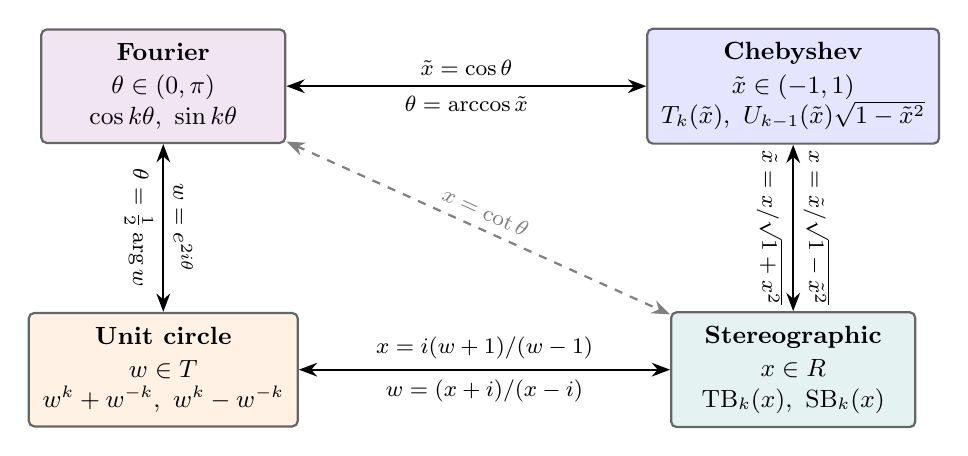
\begin{tikzpicture}[
		>=Stealth,
		every node/.style={font=\small},
		picnode/.style={
			rectangle, rounded corners=2pt, draw=black!60,
			thick, align=center, inner sep=5pt, minimum width=3.1cm
		},
		fourier/.style    ={picnode, fill=violet!10},
		chebyshev/.style  ={picnode, fill=blue!10},
		gqsp/.style       ={picnode, fill=orange!10},
		ratcheb/.style    ={picnode, fill=teal!10},
		edgelab/.style    ={font=\footnotesize, midway, sloped},
	]
	\node[fourier]   (F)  at (-4.0,  1.8) {%
		\textbf{Fourier} \\[1pt]
		$\theta \in (0,\pi)$ \\
		$\cos k\theta,\ \sin k\theta$};
	\node[chebyshev] (C)  at ( 4.0,  1.8) {%
		\textbf{Chebyshev} \\[1pt]
		$\tilde x \in (-1,1)$ \\
		$T_k(\tilde x),\ U_{k-1}(\tilde x)\sqrt{1-\tilde x^2}$};
	\node[gqsp]      (G)  at (-4.0, -1.8) {%
		\textbf{Unit circle} \\[1pt]
		$w \in \T$ \\
		$w^k+w^{-k},\ w^k-w^{-k}$};
	\node[ratcheb]   (R)  at ( 4.0, -1.8) {%
		\textbf{Stereographic} \\[1pt]
		$x \in \R$ \\
		$\TB_k(x),\ \SB_k(x)$};

	\draw[<->, thick] (F) -- (C)
	node[edgelab, above] {$\tilde x = \cos\theta$}
	node[edgelab, below] {$\theta = \arccos \tilde x$};

	\draw[<->, thick] (F) -- (G)
	node[edgelab, above] {$w = e^{2i\theta}$}
	node[edgelab, below] {$\theta = \tfrac12\arg w$};

	\draw[<->, thick] (C) -- (R)
	node[edgelab, above] {$x = \tilde x/\sqrt{1-\tilde x^2}$}
	node[edgelab, below] {$\tilde x = x/\sqrt{1+x^2}$};

	\draw[<->, thick] (G) -- (R)
	node[edgelab, above] {$x = i(w+1)/(w-1)$}
	node[edgelab, below] {$w = (x+i)/(x-i)$};

	\draw[<->, dashed, thick, gray] (F) -- (R)
	node[edgelab, above, gray] {$x = \cot\theta$};
	\end{tikzpicture}
	\caption{Four coordinates for the signal of one QSP circuit,
		with the changes of variable on the edges and the natural
		basis of each.  The rotation angle $\theta$ (Fourier) gives
		trigonometric polynomials; $\tilde x=\cos\theta$
		(Chebyshev) gives the ordinary polynomials of standard
		QSP~\cite{GSLW2019}; a point $w$ of the unit circle gives
		Laurent polynomials, as in generalized
		QSP~\cite{MotlaghWiebe2023}; and $x=\cot\theta$
		(stereographic) gives Boyd's rational Chebyshev functions
		$\TB_k(x)=\cos(k\,\mathrm{arccot}\,x)$ and
		$\SB_k(x)=\sin(k\,\mathrm{arccot}\,x)$, which are orthogonal
		on $\R$ with weight $1/(1+x^2)$~\cite{Boyd1990}.  Each
		basis function is the image of $\cos k\theta$ or
		$\sin k\theta$, so the same circuit is described in every
		box; only the stereographic coordinate covers the whole
		real line.  We use $w=e^{2i\theta}$ so that the bottom
		edge is the Cayley transform; generalized QSP uses
		$e^{i\theta}$, whose square is $w$.}
	\label{fig:charts}
\end{figure*}

% 02_projective_qsp.tex
\section{Quantum signal processing on the projective line}
\label{sec:projective}

\subsection{The qubit as a point of $\CP$}
\label{subsec:encoding}

A single-qubit pure state, taken up to global phase, is a point of
the complex projective line $\CP=\C\cup\{\infty\}$.  We fix the
identification by stereographic projection from the north pole of
the Bloch sphere,
\begin{equation}
	\mathcal{S}\colon\ket{\psi}\ \longmapsto\
	\frac{\bra{\psi}\PauliX\ket{\psi}-i\bra{\psi}\PauliY\ket{\psi}}
	{1-\bra{\psi}\PauliZ\ket{\psi}}\ \in\ \CP,
	\label{eq:decode}
\end{equation}
with inverse
\begin{equation}
	\ket{z}=\frac{1}{\sqrt{1+|z|^2}}\bigl(z\ket{0}+\ket{1}\bigr).
	\label{eq:encode}
\end{equation}
Here $z=\psi_0/\psi_1$ is the ratio of the two amplitudes: the
decoded quantity in Eq.~\eqref{eq:decode} is a \emph{ratio}, not an
amplitude, and it ranges over all of $\CP$ even though the state
stays normalized.  The map sends $z=0$ to the south pole $\ket{1}$,
$z=\infty$ to the north pole $\ket{0}$, and the equator to
$|z|=1$; its Bloch vector is
$(\langle\PauliX\rangle,\langle\PauliY\rangle,\langle\PauliZ\rangle)
=(2\re z,-2\im z,|z|^2-1)/(1+|z|^2)$.

Because decoding reads a ratio, a single-qubit gate acts on the
encoded point by a M\"obius transformation: a unitary
$\bigl(\begin{smallmatrix}a&b\\c&d\end{smallmatrix}\bigr)$ sends
$\ket{z}$ to $\ket{(az+b)/(cz+d)}$.  The Pauli gates give
$\PauliX\colon z\mapsto 1/z$, $\PauliY\colon z\mapsto -1/z$, and
$\PauliZ\colon z\mapsto -z$, and the phase gate $e^{i\phi\PauliZ}$
acts as $z\mapsto e^{2i\phi}z$.  The state $\ket{z}$ is prepared
from $\ket{0}$ by
\begin{equation}
	U_z=\frac{1}{\sqrt{1+|z|^2}}
	\begin{pmatrix} z & 1 \\ 1 & -\bar z\end{pmatrix},
	\label{eq:prep-unitary}
\end{equation}
whose columns are $\ket{z}$ and the antipodal state
$\ket{-1/\bar z}$.

\subsection{The signal operator and its base case}
\label{subsec:signal}

A QSP protocol interleaves a signal-dependent gate with tunable
phases.  In the stereographic chart the signal is a point
$z=re^{i\theta}\in\CP$, and we take as signal operator the
unnormalized matrix
\begin{equation}
	O_z=\begin{pmatrix} z & -1 \\ 1 & \bar z\end{pmatrix},
	\qquad \det O_z=1+|z|^2,
	\label{eq:Oz}
\end{equation}
whose determinant is the squared Fubini--Study norm of the
homogeneous coordinate $(z:1)$.  For a real signal $z=x\in\R$ the
operator $O_x=\bigl(\begin{smallmatrix}x&-1\\1&x\end{smallmatrix}\bigr)$
is $\sqrt{1+x^2}$ times a rotation by $\theta=\mathrm{arccot}\,x$, and
its $k$th power has entries
\begin{equation}
	O_x^{\,k}\ \propto\
	\begin{pmatrix}\cos k\theta & -\sin k\theta\\
		\sin k\theta & \cos k\theta\end{pmatrix},
	\qquad \theta=\mathrm{arccot}\,x,
	\label{eq:Ox-power}
\end{equation}
after dividing by $(1+x^2)^{k/2}$.  The matrix elements are the
\emph{rational Chebyshev functions} of Boyd~\cite{Boyd1990}
($\TB_k$ on the diagonal, $\mp\SB_k$ off it),
\begin{equation}
	\TB_k(x)=\cos(k\,\mathrm{arccot}\,x),\qquad
	\SB_k(x)=\sin(k\,\mathrm{arccot}\,x),
	\label{eq:rat-cheb}
\end{equation}
which are the images of $\cos k\theta$ and $\sin k\theta$ under the
projection $x=\cot\theta$ and are orthogonal on $\R$ with the
Cauchy weight $1/(1+x^2)$~\cite{Boyd1990,Boyd1987}.  Throughout we
fix the branch $\mathrm{arccot}\colon\R\to(0,\pi)$, so $\sin\theta>0$
and $\sqrt{1+x^2}=1/\sin\theta$ carries no sign ambiguity.  Conjugating
the normalized $k$th power by $V=\mathrm{diag}(1,i)$, that is forming
$V\,[(1+x^2)^{-k/2}O_x^{\,k}]\,V^{-1}$, gives the standard QSP signal
$W(\tilde x)^k$ of Remark~\ref{rem:basis-change}, with $+i\sin k\theta$
in \emph{both} off-diagonal entries.  Boyd writes
$\TB_k$ as $T_k$ composed with the compression
$x\mapsto x/\sqrt{1+x^2}$, since $T_k(\cos\theta)=\cos k\theta$;
Eq.~\eqref{eq:rat-cheb} is the same family.

\subsection{Completeness in the stereographic chart}
\label{subsec:completeness}

The signal operator $O_x$ and the phase gates generate a
QSP sequence whose achievable functions we now characterize.
Throughout, $P^*$ denotes the polynomial
$P^*(x)=\overline{P(\bar x)}$ obtained by conjugating the
coefficients of $P$, so that $P^*$ coincides with the complex
conjugate $\bar P$ on real arguments.  We give the real-signal case
first.

\begin{theorem}[Real stereographic QSP]
	\label{thm:real-qsp}
	For $x\in\R$ let
	$U_{\bm\phi}(x)=e^{i\phi_0\PauliZ}\prod_{j=1}^{d}O_x\,
	e^{i\phi_j\PauliZ}$.  A pair of polynomials $P,Q\in\C[x]$ is
	realizable as
	\begin{equation}
		U_{\bm\phi}(x)=
		\begin{pmatrix} P(x) & -Q^*(x)\\ Q(x) & P^*(x)\end{pmatrix}
		\label{eq:real-qsp-form}
	\end{equation}
	for some $\bm\phi\in\R^{d+1}$ if and only if
	\begin{enumerate}
		\item[(i)] $|P(x)|^2+|Q(x)|^2=(1+x^2)^d$ for all $x\in\R$;
		\item[(ii)] $P$ has parity $d\bmod 2$ and $Q$ has parity
			$(d-1)\bmod 2$;
		\item[(iii)] $\deg P\le d$ and $\deg Q\le d-1$, with the
			convention $\deg Q=-1\Leftrightarrow Q\equiv 0$.
	\end{enumerate}
\end{theorem}

The forward direction is an induction on $d$: each factor
$O_x\,e^{i\phi\PauliZ}$ raises the degree by one and multiplies the
normalization by $\det O_x=1+x^2$, which reproduces (i)--(iii).
The backward direction is the substantive half.  Condition (i) forces
$|P(i)|^2=|Q(i)|^2$ by evaluation at $x=i$; choosing the phase
$e^{2i\phi}=-iP(i)/Q^*(i)$ makes the reduced polynomials
$\widetilde P,\widetilde Q$ vanish at $x=i$, and, by parity, at
$x=-i$.  Division by $1+x^2$ then lowers the degree by one and the
induction closes.  Appendix~\ref{app:thm-real} gives the details.
The normalization (i) is the only change from the standard QSP
theorem: it is $(1+x^2)^d$ rather than $1$, because the signal
operator $O_x$ is unnormalized.  The physical gate is the unitary
$(1+x^2)^{-d/2}U_{\bm\phi}(x)\in\SU(2)$, and this global factor
cancels in the decoded ratio $P/Q$; after the basis change of
Remark~\ref{rem:basis-change} the constraint (i) becomes the
standard completeness constraint $|P|^2+|Q|^2=1$ in the compressed
variable.

Lifting the controls from $\PauliZ$-phases to arbitrary $\SU(2)$
rotations, and the signal from $\R$ to $\CP$, gives the generalized
theorem.  Its achievable class consists of \emph{bivariate}
polynomials in $z$ and $\bar z$.

\begin{theorem}[Generalized stereographic QSP]
	\label{thm:gen-qsp}
	Let $O_z$ be as in Eq.~\eqref{eq:Oz} and let
	$G_0,\dots,G_d\in\SU(2)$.  A pair $P,Q\in\C[z,\bar z]$, where
	now $P^*(z,\bar z)=\overline{P(\bar z,z)}$ conjugates coefficients
	and swaps $z\leftrightarrow\bar z$, is realizable as
	\begin{equation}
		G_d\,O_z\,G_{d-1}\,O_z\cdots O_z\,G_0
		=\begin{pmatrix} P(z,\bar z) & -Q^*(z,\bar z)\\
			Q(z,\bar z) & P^*(z,\bar z)\end{pmatrix}
		\label{eq:gen-qsp-form}
	\end{equation}
	if and only if
	\begin{enumerate}
		\item[(i)] every monomial $z^j\bar z^k$ of $P$ and $Q$ has
			$j+k\le d$;
		\item[(ii)] $P P^*+Q Q^*=(1+|z|^2)^d$.
	\end{enumerate}
\end{theorem}

The forward direction is again an induction on the number of
factors.  The backward direction reads the leading data off a
target pair and strips one layer at a time.  Applying the inverse
iterate $O_z^{-1}G_d^{-1}$ produces reduced entries
$P'=z^*\widetilde P+\widetilde Q$ and $Q'=z\widetilde Q-\widetilde
P$; requiring $1+z\bar z$ to divide both fixes the control $G_d$,
and the quotient lowers the bidegree from $d$ to $d-1$.  The
divisibility rests on a factorization in the Laurent ring:

\begin{lemma}
	\label{lem:DDstar}
	If $D\in\C[z,z^{-1}]$ satisfies $D D^*=-1$, then $D=c\,z^k$ with
	$|c|=1$ and $k$ odd.
\end{lemma}

The lemma pins down the units of the ring that can appear, and with
it the case analysis of the backward direction closes; the full
argument, including the unique-factorization step, is in
Appendix~\ref{app:thm-gen}.  Theorem~\ref{thm:gen-qsp} is the
stereographic form of generalized QSP~\cite{MotlaghWiebe2023}: the
bivariate structure in $(z,\bar z)$ is the projective-coordinate
image of the Laurent structure in $z=e^{i\theta}$, and the
Fubini--Study normalization $(1+|z|^2)^d$ is the image of the
constraint $|P|^2+|Q|^2=1$ on the unit circle.

\subsection{Three readings of the same circuit}
\label{subsec:remarks}

\begin{remark}[Reduction to standard QSP]
	\label{rem:basis-change}
	The real signal operator, once normalized, is the standard
	QSP signal conjugated by a fixed gate.  With
	$V=\mathrm{diag}(1,i)$, $\tilde x=x/\sqrt{1+x^2}$, and
	$W(\tilde x)=\bigl(\begin{smallmatrix}\tilde x &
	i\sqrt{1-\tilde x^2}\\ i\sqrt{1-\tilde x^2}&\tilde
	x\end{smallmatrix}\bigr)$ the standard signal,
	\begin{equation}
		(1+x^2)^{-1/2}O_x=V^{-1}W(\tilde x)V,
	\end{equation}
	equivalently $W(\tilde x)=V\,[(1+x^2)^{-1/2}O_x]\,V^{-1}$, and $V$
	commutes with every phase gate.  A stereographic QSP
	circuit is therefore a standard QSP circuit conjugated by a
	gate that depends on neither the signal nor the phases.  Two
	consequences follow.  The diagonal matrix element is unchanged,
	so the completeness theorem and every phase-finding
	algorithm~\cite{DongMengWhaleyEtAl2021,NiSarkarYingLin2025}
	transfer verbatim.  And the unboundedness of the decoded ratio
	is produced by the decoding step of Eq.~\eqref{eq:decode}, not
	by the circuit, whose matrix elements never exceed one.
\end{remark}

\begin{remark}[A hardware-executable read-out]
	\label{rem:measurement}
	After the basis change of Remark~\ref{rem:basis-change} the
	circuit acts on real amplitudes, so its output is a
	real-amplitude state, with a single flag qubit carrying the
	imaginary unit in the real-number formulation of
	Ref.~\cite{BarriosHita2026}.  Such states are read out by the
	$n+1$-setting protocol of
	Ref.~\cite{NguemtoLeytonOrtega2026}: computational-basis
	sampling and one Hadamard-rotated setting per qubit, which is
	minimal.  The stereographic ratio is then formed
	classically.  The read-out costs $n+1$ measurement settings and
	$\mathcal{O}(r^4/\varepsilon^2)$ shots to recover the decoded
	value at signal magnitude $r$ to absolute precision
	$\varepsilon$, the inverse projection amplifying sampling error
	by $(1+r^2)/2$ (Appendix~\ref{app:readout}).  This makes the
	decoding interface executable for order-one signals; it is a
	trade of circuit depth for shot count, not an asymptotic
	speedup, and its systematic use is left to future work.
\end{remark}

\begin{remark}[One geometry, two signal operators]
	\label{rem:two-signals}
	The stereographic map appears twice in this paper.  At the
	single-qubit scale it selects the signal operator $O_z$, whose
	powers produce the rational Chebyshev functions and whose
	achievable class the two theorems above characterize.  At the
	multi-qubit scale (Sec.~\ref{sec:stateprep}) the same map sends
	a uniform angular grid $\theta_j$ to the cotangent grid
	$y_j=L\cot\theta_j$ on $\R$, on which a diagonal walk operator
	$e^{iA}=\sum_j e^{i\theta_j}\ket{j}\!\bra{j}$ acts and the
	rational Chebyshev basis pulls back to the Fourier basis.  The
	two operators $O_z$ and $e^{iA}$ are the \emph{same geometry},
	not the same gate: they are the single- and multi-qubit
	incarnations of one stereographic construction, and the
	pairing of chart, grid, and signal operator is what turns the
	approximation theory of this section into the gate counts of
	Sec.~\ref{sec:stateprep}.
\end{remark}

% 04_limits.tex
\section{Limits of a change of variable}
\label{sec:limits}

The stereographic coordinate maps $[-1,1]$ onto the whole real line
and replaces the Chebyshev basis by the rational Chebyshev basis.
It is tempting to expect that a function which needs a high
polynomial degree in $\tilde x$ needs a low degree in $x$.  In
this section, we show that for functions of a block-encoded matrix
the degree is the same in both coordinates, and we identify the
setting in which the coordinate is of use.

We consider a block encoding $U$ of a Hermitian matrix $A/\lambda$
with eigenvalues $a_j\in[-1,1]$.  The QSVT circuit alternates $d$
applications of $U$ and $U^\dagger$ with phase rotations controlled
on the block-encoding ancillas, and it applies to the eigenvector
with eigenvalue $a_j$ a polynomial $P(a_j)$ of degree at most
$d$~\cite{GSLW2019,MartynRossiTanChuang2021}.  We recall the
argument in order to make one consequence explicit.  The
eigenvalue $a_j$ enters the circuit only through the rotation
angle $\theta_j=\arccos a_j$, and each query contributes one power
of $e^{\pm i\theta_j}$.  After $d$ queries every matrix element of
the circuit on the two-dimensional invariant subspace of $a_j$ is
therefore a trigonometric polynomial of degree at most $d$ in
$\theta_j$.  The block that the circuit encodes is a polynomial of
degree at most $d$ in $a_j=\cos\theta_j$, and the off-diagonal
elements are $\sin\theta_j=\sqrt{1-a_j^2}$ times a polynomial of
degree at most $d-1$.  Hence, the set of reachable transformations
is fixed by $d$ and is the same in every coordinate.

In particular, the expansion coefficients do not depend on the
coordinate.  Let $\theta=\arccos a$ and let
$\alpha=\cot\theta=a/\sqrt{1-a^2}$ be the stereographic coordinate
of Eq.~\eqref{eq:stereo-coord}.  Because
$T_k(a)=\TB_k(\alpha)=\cos k\theta$, every polynomial $P$ of degree
at most $d$ obeys
\begin{equation}
	P(a)=\sum_{k=0}^d c_k T_k(a)
	=\sum_{k=0}^d c_k\,\TB_k(\alpha)
	=\sum_{k=0}^d c_k\cos k\theta
	\label{eq:basis-indep}
\end{equation}
with one and the same set of coefficients $c_k$.  It follows that
the best approximation error of a target $f$ at degree $d$ is the
same in the Chebyshev, rational Chebyshev, and Fourier bases.

Since the error coincides at every degree, so does its rate of
decay with $d$.  For a target analytic near $[-1,1]$ this rate is
set by the Bernstein ellipse through the nearest singularity of
$f$~\cite[Ch.~8]{Trefethen2013}.  Under the stereographic map
these ellipses become the bipolar contours with foci $\pm i$ that
govern the convergence of rational Chebyshev
series~\cite{Boyd1990} (see also Sec.~17.7 of
Ref.~\cite{Boyd2001}), so that Boyd's convergence rate for the
rational Chebyshev series equals the Chebyshev rate.
Consequently, lower bounds for specific targets, such as those of
Sherstov~\cite{Sherstov2013} and the adversary bound of
Laneve~\cite{Laneve2025}, are unchanged by the change of variable.

The argument above takes the sample
points of the polynomial as given: they are the eigenvalues $a_j$
of the matrix $A$.  In state preparation, in contrast, there is no
given matrix.  The task is to write prescribed numbers $f(y_j)$
into the amplitudes of a register, and the points $y_j$ at which
$f$ is sampled are part of the design.  The argument does not
constrain this choice.  In Sec.~\ref{sec:stateprep}, we use this
freedom and choose the points such that $f$, written in the angle
variable, is a smooth function sampled on a uniform grid.

% 05_state_prep.tex
\section{State preparation on unbounded domains}
\label{sec:stateprep}

The no-go of Sec.~\ref{sec:limits} closes the door on chart change
within block encoding.  We now open a different one.  Pairing the
stereographic chart with a cotangent grid and a diagonal
Fourier-type signal operator prepares a quantum state encoding a
function $f\colon\R\to\C$ on the whole real line, at a cost set only
by the shape of $f$ after pullback to the circle.  The signal
operator is a walk with prescribed eigenphases, not a block
encoding of a Hermitian operator, so Proposition~\ref{prop:nogo}
does not apply.

\subsection{The cotangent grid}
\label{subsec:grid}

We prepare an $N=2^n$-dimensional state
\begin{equation}
	\ket{\Psi_f}=\frac{1}{\mathcal{N}_f}\sum_{j=0}^{N-1}f(y_j)\ket{j},
	\qquad \mathcal{N}_f=\Bigl(\textstyle\sum_j|f(y_j)|^2\Bigr)^{1/2},
	\label{eq:target-state}
\end{equation}
on the \emph{cotangent grid}
\begin{equation}
	y_j=L\cot\theta_j,\qquad \theta_j=\frac{\pi(2j+1)}{2N},
	\qquad j=0,\dots,N-1,
	\label{eq:cot-grid}
\end{equation}
the image under $y=L\cot\theta$ of a uniform angular grid.  The
half-integer shift keeps every point interior to $(0,\pi)$.  The
map parameter $L>0$ sets the density of points near $y=0$; the grid
clusters at the origin and thins in the tails, the reverse of the
Chebyshev grid on $[-1,1]$.  Its extent is $|y|\lesssim 2LN/\pi$,
which grows exponentially with $n$.  The cotangent grid thus ties
the represented range to the qubit count $n$; it does not
\emph{eliminate} truncation, but replaces a user-chosen radius by a
range fixed by the resource $n$, beyond which the unrepresented
tail mass is exponentially small in $n$ for the targets below.

\subsection{The Boyd class}
\label{subsec:boyd}

Given $f\colon\R\to\C$, its stereographic pullback is
$g(\theta)=f(L\cot\theta)$.  Because $\cot$ has period $\pi$, $g$ is
$\pi$-periodic, so its Fourier series contains only the harmonics
$\cos 2k\theta$ and $\sin 2k\theta$.  The rational Chebyshev
functions of Eq.~\eqref{eq:rat-cheb} satisfy
$\TB_k(y_j;L)=\cos k\theta_j$ and $\SB_k(y_j;L)=\sin k\theta_j$, so
a degree-$d$ rational Chebyshev approximation of $f$ on $\R$ is a
degree-$d$ trigonometric approximation of $g$ on the circle.

\begin{definition}[Boyd class~\cite{Boyd1990}]
	\label{def:boyd}
	$f$ belongs to $\mathcal{B}(L)$ if it is free of singularities
	on the real axis and its pullback $g$ has Fourier coefficients
	obeying $|a_k|,|b_k|\le C\exp(-q k^\sigma)$ for some $C,q>0$ and
	$\sigma\in(0,1]$.
\end{definition}

By Boyd's theorem~\cite{Boyd1990}, $f\in\mathcal{B}(L)$ with
\emph{geometric} rate ($\sigma=1$) if and only if $g$ extends
analytically to a neighborhood of the real $\theta$-axis, which
requires $f$ analytic near the real $y$-axis \emph{and} analytic at
infinity, i.e., possessing a convergent expansion in $1/y$.  The
degree for $L^\infty$-error $\delta$ is then
$d_\delta=\mathcal{O}(\log(1/\delta))$.  When $f$ has an essential
singularity at infinity the pullback has an essential singularity
at the endpoint $\theta=0$, the analyticity strip collapses, and
the rate is \emph{subgeometric}, $\sigma<1$, with
$d_\delta=\mathcal{O}((\log(1/\delta))^{1/\sigma})$.  Two targets
of interest are subgeometric with $\sigma=1/2$: the Gaussian, whose
essential singularity at infinity is standard, and the hyperbolic
secant.  For $\mathrm{sech}(L\cot\theta)$ the poles of $\mathrm{sech}$
pull back to points $\theta_m$ with $|\im\theta_m|\to 0$ as
$m\to\infty$, accumulating on the real axis, so no strip exists and
the coefficients decay as $\exp(-c\sqrt{k})$
(Appendix~\ref{app:sech}).  The hyperbolic secant is therefore
\emph{not} in the geometric class, contrary to a natural reading of
its exponential decay; exponential decay on $\R$ is necessary but
not sufficient for geometric convergence, which needs analyticity
at infinity.

\subsection{Filling fraction}
\label{subsec:filling}

The success probability of the preparation is governed by the
filling fraction
\begin{equation}
	\mathcal{F}_g^{[N]}=\frac{1}{\sqrt{N}}\cdot
	\frac{\bigl(\sum_{j=0}^{N-1}|g(\theta_j)|^2\bigr)^{1/2}}{|g|_{\max}},
	\qquad |g|_{\max}=\max_{(0,\pi)}|g|.
	\label{eq:filling}
\end{equation}

\begin{lemma}[Continuous limit]
	\label{lem:filling}
	If $g\in C^2(0,\pi)$ with $|g|_{\max}<\infty$ attained at an
	interior point, then
	\begin{equation}
		\mathcal{F}_g^{[N]}=\mathcal{F}_g^{[\infty]}+\mathcal{O}(N^{-2}),
		\qquad
		\mathcal{F}_g^{[\infty]}=\frac{\|g\|_{L^2(0,\pi)}}
		{\sqrt{\pi}\,|g|_{\max}}.
		\label{eq:filling-limit}
	\end{equation}
\end{lemma}

The sum in Eq.~\eqref{eq:filling} is the midpoint rule for
$(1/\pi)\int_0^\pi|g|^2$ on the grid $\theta_j$, whose error is
$\mathcal{O}(N^{-2})$ for $g\in C^2$; the square root and the
$\mathcal{O}(N^{-2})$ agreement of the discrete and continuous
maxima preserve the rate (Appendix~\ref{app:filling}).  The
continuous limit depends only on the shape of $g$ and on no
truncation parameter.  For the targets below, $g$ is $C^\infty$
with bounded derivatives, so the discrete and continuous filling
fractions agree to $1+\mathcal{O}(2^{-n})$.

\subsection{Algorithm and main result}
\label{subsec:algorithm}

The algorithm has three stages.  \emph{Classical preprocessing}
computes the pullback $g$, normalizes to $\hat g=g/|g|_{\max}$ with
$|\hat g|\le 1$, and approximates $\hat g$ by a degree-$d_\delta$
trigonometric polynomial $\tilde g$ to $L^\infty$-error $\delta$;
because $g$ is $\pi$-periodic, $\tilde g$ is built from even
harmonics on the full circle, so $|\tilde g|\le 1+\delta$ holds on
all of $\T$ and is restored to $|\tilde g|\le 1$ by rescaling with
$1/(1+\delta)$.  The QSP phases follow from any standard
solver~\cite{DongMengWhaleyEtAl2021,BerntsonSunderhauf2024,NiSarkarYingLin2025}
at cost negligible against the circuit for the targets here.
\emph{The Fourier-QET circuit} uses the diagonal signal operator
\begin{equation}
	e^{iA}=\sum_{j=0}^{N-1}e^{i\theta_j}\ket{j}\!\bra{j},\qquad
	\theta_j=\frac{\pi(2j+1)}{2N},
	\label{eq:qet-signal}
\end{equation}
whose phase $\theta_j=\pi/(2N)+\sum_{k}j_k\pi 2^k/N$ decomposes over
the bits of $j$, so $e^{iA}$ costs $\mathcal{O}(n)$ elementary
gates: $n$ single-qubit $R_z$ rotations, one on each qubit $k$ with
angle $\pi 2^k/N$, and one global phase.  With
$d_\delta$ applications of $e^{\pm iA}$ and $\mathcal{O}(d_\delta)$
ancilla rotations, the circuit block-encodes the diagonal
$D_{\tilde g}=\sum_j\tilde g(\theta_j)\ket{j}\!\bra{j}$.
\emph{Amplitude amplification} boosts the flagged block to unity in
$\mathcal{O}(1/\mathcal{F}_{\tilde g}^{[N]})$ rounds with one extra
ancilla.

\begin{theorem}[Stereographic state preparation]
	\label{thm:stateprep}
	Let $f\in\mathcal{B}(L)$ and let a degree-$d_\delta$
	trigonometric polynomial approximate $\hat g$ to $L^\infty$-error
	$\delta=\tfrac12\varepsilon\cdot
	\min(\mathcal{F}_g^{[N]},\mathcal{F}_{\tilde g}^{[N]})$ on the
	circle.  The algorithm prepares a state $\varepsilon$-close in
	trace distance to $\ket{\Psi_f}$ using
	\begin{equation}
		\mathcal{O}\!\left(\frac{n\,d_\delta}{\mathcal{F}_{\tilde g}^{[N]}}\right)
		\text{ gates}
		\label{eq:stateprep-cost}
	\end{equation}
	and at most two ancilla qubits, one for the signal and one for
	amplitude amplification.  For the geometric class
	$d_\delta=\mathcal{O}(\log(1/\varepsilon))$ and the cost is
	$\mathcal{O}(n\log(1/\varepsilon)/\mathcal{F}_g^{[\infty]})$;
	for the subgeometric class
	$d_\delta=\mathcal{O}((\log(1/\varepsilon))^{1/\sigma})$.
\end{theorem}

The proof (Appendix~\ref{app:stateprep}) applies the QSP
completeness theorem on the full circle, evaluates the resulting
diagonal on $\ket{+}^{\otimes n}$, and converts the $L^\infty$
approximation error to trace distance through the filling fraction;
the choice $\delta=\tfrac12\varepsilon\min(\mathcal{F}_g^{[N]},
\mathcal{F}_{\tilde g}^{[N]})$ controls both filling fractions
without assuming an order between them.  A degree-$d_\delta$
trigonometric polynomial has $2d_\delta+1\le N$ degrees of freedom
on the $N$ grid points, so no aliasing enters while
$d_\delta=\mathcal{O}((\log(1/\varepsilon))^{1/\sigma})$ stays below
$N/2$, which holds at every qubit count of interest.

\subsection{Examples}
\label{subsec:examples}

For the Lorentzian $f(y)=1/(1+y^2)$ with $L=1$, the pullback is
\begin{equation}
	g(\theta)=\frac{1}{1+\cot^2\theta}=\sin^2\theta
	=\tfrac12(1-\cos 2\theta),
\end{equation}
a trigonometric polynomial of degree two with no approximation
error, $\delta=0$.  The filling fraction is
$\mathcal{F}_g^{[\infty]}=\sqrt{3/8}\approx 0.612$, one round of
amplitude amplification suffices, and the cost is $\mathcal{O}(n)$.
More generally $1/(1+y^2)^s$ for integer $s$ pulls back to
$\sin^{2s}\theta$, a trigonometric polynomial of degree $2s$, so the
whole family has cost independent of the represented range.

For the hyperbolic secant, $\sigma=1/2$ (Sec.~\ref{subsec:boyd}),
so $d_\delta=\mathcal{O}(\log^2(1/\varepsilon))$ and the cost is
$\mathcal{O}(n\log^2(1/\varepsilon))$.  For the Gaussian
$e^{-\beta y^2/2}$ with $L=1/\sqrt{\beta}$, the pullback
$e^{-\cot^2\theta/2}$ is subgeometric with $\sigma=1/2$, giving
$\mathcal{O}(n\log^2(1/\varepsilon))$.  For the shifted Lorentzian
$1/((y-a)^2+b^2)$ the pullback is meromorphic in $e^{i\theta}$ with
poles at distance $\mathcal{O}(\min(b,L)/L)$ from the real axis,
giving geometric convergence at rate
$d_\delta=\mathcal{O}((L/b)\log(1/\varepsilon))$; centered and at
natural width ($a=0$, $b=L$) this reduces to
$\mathcal{O}(\log(1/\varepsilon))$.

\subsection{Quadrature-weighted preparation}
\label{subsec:quadrature}

Downstream tasks that consume the state as an inner product
$\langle f\mid g\rangle\approx\int_\R f(y)\overline{g(y)}\,dy$ need
the cotangent-grid Jacobian $|dy/d\theta|=L/\sin^2\theta$.  Encoding
the weighted amplitudes $f(y_j)/\sin\theta_j$ builds the Jacobian
in:
\begin{equation}
	\int_{-\infty}^{\infty}\! f(y)\,dy
	=\int_0^\pi\! f(L\cot\theta)\frac{L}{\sin^2\theta}\,d\theta
	\approx\frac{\pi L}{N}\sum_{j=0}^{N-1}\frac{g(\theta_j)}{\sin^2\theta_j}.
	\label{eq:quadrature}
\end{equation}
For the Lorentzian with $L=1$ the weighted amplitude is
$f(y_j)/\sin\theta_j=\sin\theta_j$, again a degree-one trigonometric
polynomial, so the quadrature-weighted preparation also costs
$\mathcal{O}(n)$.  More generally, the weighted variant has the same
asymptotic cost as the unweighted one whenever $g(\theta)/\sin^2\theta$
remains in a class with convergent Fourier expansion, which holds for
$f(y)=\mathcal{O}(y^{-2})$ at infinity.

\subsection{Comparison}
\label{subsec:comparison}

Three families of methods are directly comparable.  The QSVT
pipeline of McArdle, Gily\'en, and
Berta~\cite{McArdleGilyenBerta2025} approximates $f$ on a truncated
interval $[-L_{\mathrm{trunc}},L_{\mathrm{trunc}}]$ through
$y=L_{\mathrm{trunc}}\sin\theta$; the user picks
$L_{\mathrm{trunc}}$ to balance the truncation tail against the
polynomial degree.  The Schmidt-decomposition circuit of
Gonz\'alez-Conde \emph{et al.}~\cite{GonzalezCondeEtAl2020} and the
matrix-product-state construction of Sano and
Hamamura~\cite{SanoHamamura2025} prepare Lorentzians and other
smooth densities at linear depth on a finite domain.
Table~\ref{tab:comparison} collects the gate counts;
Appendix~\ref{app:table} derives each entry under one accounting,
gate count $=n\times$ (polynomial degree) $\times\,1/\mathcal{F}$.

\begin{table*}[t]
	\caption{Gate complexity for preparing a state encoding $f(y)$
		on $n$ qubits to trace distance $\varepsilon$.  The QSVT
		column~\cite{McArdleGilyenBerta2025} is evaluated at the
		truncation radius that balances the tail against the degree;
		for the Lorentzian this is $L_{\mathrm{trunc}}=\varepsilon^{-2/3}$,
		since the truncated-state trace distance scales as the square
		root of the discarded $L^2$-mass.  The linear-depth Lorentzian
		preparations of Refs.~\cite{GonzalezCondeEtAl2020}~(GC)
		and~\cite{SanoHamamura2025}~(SH) are listed where they apply.
		The stereographic method carries no truncation radius; its
		cost is set by the shape-only filling fraction.  Derivations
		are in Appendix~\ref{app:table}.}
	\label{tab:comparison}
	\begin{ruledtabular}
		\begin{tabular}{lllll}
			Target $f(y)$ & QSVT~\cite{McArdleGilyenBerta2025}
			& GC~\cite{GonzalezCondeEtAl2020}
			& SH~\cite{SanoHamamura2025}
			& Stereographic (this work)\\
			\hline
			$1/(1+y^2)$
			& $\mathcal{O}(n\,\varepsilon^{-1}\log\tfrac1\varepsilon)$
			& $\mathcal{O}(n)$ & $\mathcal{O}(n)$ & $\mathcal{O}(n)$\\[2pt]
			$\mathrm{sech}(y)$
			& $\mathcal{O}(n\log^{5/2}\tfrac1\varepsilon)$
			& n.a. & n.a. & $\mathcal{O}(n\log^{2}\tfrac1\varepsilon)$\\[2pt]
			$e^{-\beta y^2/2}$
			& $\tilde{\mathcal{O}}(n\log^{5/4}\tfrac1\varepsilon)$
			& $\mathcal{O}(n)$ & $\mathcal{O}(n)$
			& $\mathcal{O}(n\log^{2}\tfrac1\varepsilon)$\\[2pt]
			$1/((y-a)^2+b^2)$
			& $\mathcal{O}(\tfrac{n}{b}\varepsilon^{-1}\log\tfrac1\varepsilon)$
			& $\mathcal{O}(n)$ & n.a.
			& $\mathcal{O}(\tfrac{nL}{b}\log\tfrac1\varepsilon)$
		\end{tabular}
	\end{ruledtabular}
\end{table*}

For the centered Lorentzian the stereographic method gains a factor
$\varepsilon^{-1}\log(1/\varepsilon)$ over the QSVT pipeline, a
polynomial-in-$\varepsilon$ advantage that comes from the exact
degree-two pullback and the absence of a truncation radius; it ties
the linear-depth preparations of
Refs.~\cite{GonzalezCondeEtAl2020,SanoHamamura2025} at
$\mathcal{O}(n)$, where the stereographic gain is instead
qualitative: one algorithm covers Boyd's class without the
per-target redesign those constructions require, and it removes the
truncation radius.  For the hyperbolic secant it improves on the
QSVT pipeline by $\log^{1/2}(1/\varepsilon)$.  For Gaussians it is
slower than every baseline, by $\log^{3/4}(1/\varepsilon)$ against
the QSVT pipeline and by a logarithmic factor against the
linear-depth methods.  The two-ancilla budget is one to two qubits
below the QSVT pipeline, which uses four in the general case and
three under parity, because the diagonal signal $e^{iA}$ needs no
separate block-encoding ancilla.  Reciprocally, the linear-depth
methods prepare truncated Lorentzians exactly and extend to targets
outside Boyd's class; we claim a complementary route, not a
dominating one.  The output lives on the cotangent grid;
applications requiring a different grid need a regridding step we do
not analyze.  Convergence data for these targets appear in
Fig.~\ref{fig:convergence}.

\begin{figure*}[t]
	\centering
	\includegraphics[width=\textwidth]{figures/convergence_comparison.pdf}
	\caption{$L^\infty$ approximation error versus polynomial degree
		$d$ for the four targets, comparing the rational Chebyshev
		expansion on $\R$ (this work) with truncated Chebyshev
		expansions on $[-L,L]$ at several $L$.  For the Lorentzian
		and shifted Lorentzian the rational basis converges at a
		rate independent of the represented range, while the
		truncated expansions degrade as $L$ grows; for the
		hyperbolic secant and Gaussian the subgeometric rate
		$\exp(-c\sqrt d)$ is visible as the characteristic downward
		curvature, matching the classification of
		Sec.~\ref{subsec:boyd}.}
	\label{fig:convergence}
\end{figure*}

The Lorentzian speedup does not contradict the no-go of
Sec.~\ref{sec:limits}.  That obstruction constrains polynomials of
a block-encoded eigenvalue; here the signal is a walk with
prescribed cotangent-spaced eigenphases and the basis is the
rational Chebyshev family on $\R$.  The chart change alone buys
nothing; the chart paired with the matching grid and signal
operator is what buys the gate savings.

% 06_discussion.tex
\section{Conclusions}
\label{sec:discussion}

To conclude, we have formulated QSP in the stereographic
coordinate $x=\cot\theta$, which covers the whole real line, and
have used it to prepare functions on the real line as quantum
states without truncation.  In this coordinate a QSP sequence is
the standard sequence conjugated by a fixed gate, so that its
phases follow from the standard theory.  An unbounded value is
read out as the ratio of two bounded amplitudes, with a number of
shots which grows as the fourth power of that value.  For functions of a block-encoded matrix, the expansion
coefficients and the approximation error at every degree coincide
in every coordinate, so that the known bounds apply unchanged.

We have found that the benefit of the coordinate lies in the
choice of sample points for state preparation.  On the cotangent grid, a function weighted
by the square root of the grid spacing becomes a function on a
uniform grid of angles, and the prepared state represents the
original function in the norm of $L^2(\R)$ with the approximation
error as its only error.  The state is the quantum Fourier
transform of a short coefficient vector and needs no ancilla.
Alternatively, it is prepared by a QSP circuit whose signal is the
Cayley transform of the position operator of the grid.

We have shown that the length of the coefficient vector does not
depend on the error for the Lorentzian and the related amplitudes with algebraic tails, for
which a uniform grid needs a degree that grows as a power of the
inverse error.  For the hyperbolic secant and the Gaussian, in
turn, the length grows polylogarithmically with the inverse error,
and the cotangent grid is more economical for the former and
equivalent for the latter, where its cost with amplitude
amplification lies between $0.9$ and $1.3$ times that of the QSVT
pipeline.

Three properties of the construction set the scope of these
results.  First, the state
represents the function by interpolation in the rational Chebyshev
basis and not by samples on a uniform grid.  A single qubit, for
instance, already represents the Lorentzian exactly.  Hence, a
task which needs the amplitudes on a uniform grid requires a
regridding step, which we leave for future work.
Second, the grid is dense at one point only.  Two Lorentzians of
width $b$ separated by $2|a|\gg b$ therefore need a degree which
grows as $|a|/b$, against $d=1$ for a single one.  Third, the construction requires a signal
operator whose eigenphases we choose.  For a block-encoded
Hamiltonian with given eigenvalues the Cayley transform costs a
linear solve~\cite{DelCorso2026}, and the approximation error
is then the same in every coordinate (Sec.~\ref{sec:limits}).

A natural next step is to identify tasks which consume the state
through the overlaps and expectation values of
Eqs.~\eqref{eq:quadrature} and~\eqref{eq:expectation}, which are exact integrals over the
real line.  One candidate is amplitude estimation of expectation
values under Cauchy and Student $t$ distributions, whose square
roots are the states prepared exactly in
Sec.~\ref{subsec:examples} and for which a uniform grid requires
truncation.


\begin{acknowledgments}
	This material is based upon work supported by the U.S.\
	Department of Energy, Office of Science, Accelerated Research
	in Quantum Computing, Fundamental Algorithmic Research toward
	Quantum Utility (FAR-Qu).
\end{acknowledgments}

\section*{Data availability}
The reference implementation and data supporting the numerical
results, including the coefficient-decay study of
Appendix~\ref{app:sech} and the cost comparison of
Sec.~\ref{subsec:comparison}, will be deposited in a public repository
upon publication.

\appendix

\section{Direct proof of Theorem~\ref{thm:real-qsp}}
\label{app:thm-real}

The proof in Sec.~\ref{subsec:signal} reduces the theorem to the
standard one.  Here we prove it directly in the variable $x$, by
induction on $d$.

\emph{Forward direction.}  For $d=0$,
$e^{i\phi_0\PauliZ}=\mathrm{diag}(e^{i\phi_0},e^{-i\phi_0})$ has
$P=e^{i\phi_0}$, $Q\equiv 0$, and $|P|^2+|Q|^2=1=(1+x^2)^0$, with
$\deg P=0$ and $\deg Q=-1$.  Assume the form~\eqref{eq:real-qsp-form}
at degree $d-1$.  Multiplying by $e^{i\phi_d\PauliZ}O_x$ gives
\begin{equation}
	\begin{pmatrix}\widetilde P\\ \widetilde Q\end{pmatrix}
	=\begin{pmatrix} e^{i\phi_d}(xP-Q)\\ e^{-i\phi_d}(xQ+P)\end{pmatrix},
\end{equation}
so that $e^{i\phi_d\PauliZ}O_x U_{\bm\phi}=
\bigl(\begin{smallmatrix}\widetilde P&-\widetilde Q^*\\
\widetilde Q&\widetilde P^*\end{smallmatrix}\bigr)$.  Direct expansion
gives
$|\widetilde P|^2+|\widetilde Q|^2=|xP-Q|^2+|xQ+P|^2
=(1+x^2)(|P|^2+|Q|^2)=(1+x^2)^d$, the cross terms cancelling.  Since
$x$ multiplies $P$ on the diagonal and $Q$ on the off-diagonal,
$\deg\widetilde P\le d$ and $\deg\widetilde Q\le d-1$, and the
parities shift by one as required.

\emph{Backward direction.}  Let $P,Q$ satisfy (i)--(iii).  For
real $x$, $|P(x)|^2=P(x)P^*(x)$ with $P^*(x)=\overline{P(\bar x)}$,
so (i) states that the polynomial $PP^*+QQ^*-(1+x^2)^d$ vanishes on
$\R$.  A polynomial that vanishes on $\R$ is identically zero, so
$P(x)P^*(x)+Q(x)Q^*(x)=(1+x^2)^d$ holds for all complex $x$, and in
particular at $x=i$, where the right side vanishes.  There
$P^*(i)=\overline{P(-i)}=(-1)^d\overline{P(i)}$ and
$Q^*(i)=(-1)^{d-1}\overline{Q(i)}$ by the parities (ii), so the
identity at $x=i$ reads $(-1)^d\bigl(|P(i)|^2-|Q(i)|^2\bigr)=0$,
that is, $|P(i)|^2=|Q(i)|^2$.  The outermost factor
$e^{i\phi\PauliZ}O_x$ is removed by applying
$(1+x^2)\,O_x^{-1}e^{-i\phi\PauliZ}$, with
$(1+x^2)\,O_x^{-1}=\bigl(\begin{smallmatrix}x&1\\-1&x
\end{smallmatrix}\bigr)$, which gives
\begin{equation}
	\begin{pmatrix}\widetilde P\\ \widetilde Q\end{pmatrix}
	=\begin{pmatrix} x\,e^{-i\phi}P+e^{i\phi}Q\\
		-e^{-i\phi}P+x\,e^{i\phi}Q\end{pmatrix}.
\end{equation}
If $Q(i)\neq 0$, choose $\phi$ with $e^{2i\phi}=-iP(i)/Q(i)$, which
has unit modulus by $|P(i)|=|Q(i)|$.  Then
$\widetilde P(i)=e^{-i\phi}\bigl(iP(i)+e^{2i\phi}Q(i)\bigr)=0$, and
$\widetilde Q(i)=i\,\widetilde P(i)=0$.  By the parities (ii),
$\widetilde P(-i)=(-1)^{d+1}\widetilde P(i)$ and
$\widetilde Q(-i)=(-1)^{d}\widetilde Q(i)$, so both vanish also at
$x=-i$ and $1+x^2$ divides $\widetilde P$ and $\widetilde Q$.  Since
$|\widetilde P|^2+|\widetilde Q|^2=(1+x^2)^{d+1}$, the
quotients $\widehat
P=\widetilde P/(1+x^2)$, $\widehat Q=\widetilde Q/(1+x^2)$ satisfy
$|\widehat P|^2+|\widehat Q|^2=(1+x^2)^{d-1}$ with degrees $d-1$ and
$d-2$.  If instead $Q(i)=0$, then $P(i)=0$ as well, $1+x^2$
already divides both, and any $\phi$ works.  Recursing to $d=0$
yields the phases $\bm\phi$.\qed

\section{Subgeometric pullbacks of the hyperbolic secant and the Gaussian}
\label{app:sech}

The pullback $g(\theta)=\mathrm{sech}(L\cot\theta)$ inherits the
singularities of $\mathrm{sech}$, whose poles sit at
$y=i\pi(2\ell+1)/2$.  Solving $L\cot\theta=i\pi(2\ell+1)/2$ with
$w=e^{2i\theta}$ gives $\cot\theta=i(w+1)/(w-1)$, so
$w=(C+1)/(C-1)$ with $C=\pi(2\ell+1)/(2L)$, which exceeds one for
$\pi(2\ell+1)>2L$; then $\theta_\ell=-\tfrac{i}{2}\log w$ is purely
imaginary with
\begin{equation}
	\begin{split}
		|\im\theta_\ell| &=\tfrac12\log\frac{C+1}{C-1}
		=\frac{1}{C}+\mathcal{O}(C^{-3})\\
		&=\frac{2L}{\pi(2\ell+1)}+\mathcal{O}(\ell^{-3})
		\ \xrightarrow{\ell\to\infty}\ 0.
	\end{split}
\end{equation}
The singularities accumulate on the real $\theta$-axis at
$\theta=0$.  Hence, $g$ admits no analyticity strip and its Fourier
coefficients cannot decay geometrically.  Steepest descent on
$\int e^{-L/\theta}\cos(2m\theta)\,d\theta$, the endpoint form of $g$
near $\theta=0$ where $g\sim 2e^{-L/\theta}$, gives
$|a_m|\sim\exp(-c\sqrt{m})$ for the coefficients of
Eq.~\eqref{eq:boyd-bound}, that is, $\sigma=1/2$.

The Gaussian has the same mechanism with a stronger singularity.
Its pullback behaves as $\exp(-L^2/2\theta^2)$ near $\theta=0$.
For $\int e^{-\kappa/\theta^2+2im\theta}d\theta$ the saddle point
is at $\theta_\star^3=i\kappa/m$, where the exponent equals
$-3\kappa/\theta_\star^2$, whose real part is
$-\tfrac32\kappa^{1/3}m^{2/3}$.  The coefficients $a_m$ therefore
decay as $\exp(-c\,m^{2/3})$, that is, $\sigma=2/3$.  For $\kappa=1$
this reproduces Boyd's result $\exp(-1.5\,m^{2/3})
\cos(2.60\,m^{2/3}+\pi/4)$ for $\exp(-\cot^2\theta)$, including the
oscillation frequency $1.5\sqrt3\approx 2.60$~\cite[Eq.~(2.11)]{Boyd2001}.

Next, we let the map parameter grow with the degree.  At fixed
$L$ the rate derived above holds for the harmonics $k\gg\beta L^2$
of $G$.  The lower harmonics are governed by the peak of $G$ at
$\theta=\pi/2$, where
$G\approx\exp[-\beta L^2(\theta-\pi/2)^2/2]$, and they decay as
$\exp(-k^2/2\beta L^2)$.  A larger $L$ thus raises the first rate,
whose exponent grows as $L^{2/3}$, and lowers the second.  With
$L=\lambda\sqrt{d}$ both exponents are of order $d$ at the
truncation degree.  The coefficient of $e^{id\theta}$ in $G$ is then
$\pi^{-1}\int_0^\pi\exp\{d[-\beta\lambda^2\cot^2\theta/2
-i\theta]\}\,d\theta/\sin\theta$, whose exponent is $d$ times a
function independent of $d$, and the same holds for the harmonics
$k>d$ at fixed $k/d$.  Steepest descent therefore gives an error
$\exp(-\varphi(\lambda)\,d)$ up to a factor polynomial in $d$.
For $\beta=1$ and $\lambda=0.86$, we evaluated the $L^2$ error
of the truncated series in extended-precision arithmetic and
obtained $-\log\varepsilon/d=0.457$, $0.454$, and $0.446$ at $d=81$, $161$,
and $321$; the values $\lambda=0.7$, $0.8$, and $0.95$ give smaller
rates at $d=161$ and $321$.
The numerical coefficient decay for both targets is generated by
the reference implementation (see Data availability).

\section{Proof of Theorem~\ref{thm:stateprep}}
\label{app:filling}
\label{app:stateprep}

We prove the statements of the theorem in turn, starting with the
two circuits.  Write $p=\sum_k c_k e^{ik\theta}$, the sum running
over $|k|\le d$ with $k$ of the parity of $d$.  Then
$p(\theta)=e^{-id\theta}q(e^{2i\theta})$ with
$q(w)=\sum_{m=0}^{d}c_{2m-d}\,w^m$, which is
Eq.~\eqref{eq:factorization}, and
$|q(e^{2i\theta})|=|p(\theta)|\le1$ on the unit circle.

\emph{Fourier loading.}  With
$e^{2im\theta_j}=e^{i\pi m/N}e^{2\pi imj/N}$, the
factorization gives Eq.~\eqref{eq:fourier-loading}.  The quantum
Fourier transform maps $\ket{m}$ to
$N^{-1/2}\sum_je^{2\pi imj/N}\ket{j}$, so it maps the normalized
state with amplitudes proportional to $c_{2m-d}\,e^{i\pi m/N}$,
$m=0,\dots,d$, to the state with amplitudes proportional to
$q(e^{2i\theta_j})$.  The layer $e^{-idA}$ of $n$ single-qubit
phase rotations, with $A=\sum_j\theta_j\ket{j}\!\bra{j}$, completes
$p(\theta_j)$.  A state on $\lceil\log_2(d+1)\rceil$ qubits is
prepared with $\mathcal{O}(d)$ gates.  In the transform, each of
the $n$ output qubits receives one Hadamard gate and one
controlled rotation from every less significant input qubit.  The
input qubits beyond the first $\lceil\log_2(d+1)\rceil$ are in
the state $\ket{0}$, so that their rotations act trivially and
are omitted.  The transform therefore costs
$\mathcal{O}(n\log d)$ gates, and $\mathcal{O}(n)$ for $d\le1$.
The layer costs $n$, which is count (a).

\emph{QSP circuit.}  By the
completeness theorem of generalized
QSP~\cite[Cor.~5]{MotlaghWiebe2023}, there are $d+1$ rotations of the
signal ancilla which, interleaved with $d$ applications of the
controlled $e^{2iA}$, place $q(e^{2iA})$ in the flagged block.
Since $A$ is diagonal, this block is
$\sum_j q(e^{2i\theta_j})\ket{j}\!\bra{j}$, and multiplication by
$e^{-idA}$ gives
$D_p=\sum_j p(\theta_j)\ket{j}\!\bra{j}$.

\emph{Amplitude.}  Applied to $\ket{+}^{\otimes n}$, the QSP circuit
flags the vector $N^{-1/2}\sum_j p(\theta_j)\ket{j}$, whose norm is
$(N^{-1}\sum_j|p(\theta_j)|^2)^{1/2}$.  By
Lemma~\ref{lem:quadrature} with $r=p$, which applies because
$d<N$, this norm equals $\|p\|/\sqrt\pi=\mathcal{F}_p$.  The
harmonics of one parity are orthogonal on $(0,\pi)$, so
$\|p\|^2=\pi\sum_k|c_k|^2$ and $\mathcal{F}_p$ is known from the
coefficients.  Exact amplitude
amplification~\cite{BrassardHoyerMoscaTapp2002,McArdleGilyenBerta2025}
with $\mathcal{O}(1/\mathcal{F}_p)$ rounds and one further ancilla
then prepares the normalized state with certainty.

\emph{Gate count of the QSP circuit.}  Each controlled $e^{2iA}$ costs
$\mathcal{O}(n)$ gates, the block-encoding uses $d$ of them and
the layer $e^{-idA}$ of $n$ rotations, and amplitude amplification
calls the block-encoding and its inverse
$\mathcal{O}(1/\mathcal{F}_p)$ times.  The product is
Eq.~\eqref{eq:stateprep-cost}, which is count (b).

\emph{Error.}  The prepared amplitudes are
$p(\theta_j)/(\sqrt{N/\pi}\,\|p\|)$ for either circuit, and the
state represents the
function $f_p$ of Eq.~\eqref{eq:represented}.  The unitary map of
Eq.~\eqref{eq:weighted} sends $f/\|f\|$ to $G/\|G\|$ and $f_p$ to
$p/\|p\|$, so the $L^2(\R)$ distance of the first pair equals the
$L^2(0,\pi)$ distance of the second, which is
Eq.~\eqref{eq:error-identity}.

\emph{Boyd class.}  Let $g=\sum_m a_m w^m$ with $w=e^{2i\theta}$
and $|a_m|\le C\exp(-\mu|m|^\sigma)$.  If $f$ vanishes at infinity,
then $g(0)=\sum_m a_m=0$ and $g=\sum_m a_m(w^m-1)$.  With
$1/\sin\theta=2ie^{i\theta}/(w-1)$ and
$(w^m-1)/(w-1)=\sum_{j=0}^{m-1}w^j$ for $m>0$, and the
corresponding sum for $m<0$,
\begin{equation}
	G=2i\sum_{j\ge0}\Bigl(\sum_{m>j}a_m\Bigr)e^{i(2j+1)\theta}
	-2i\sum_{j<0}\Bigl(\sum_{m\le j}a_m\Bigr)e^{i(2j+1)\theta}.
\end{equation}
The coefficients $c_k$ of $G$ are thus tail sums of the $a_m$ and
obey $|c_k|=\mathcal{O}(|k|^{1-\sigma}\exp(-\mu|k/2|^\sigma))$.  Let
$p_d$ be the sum over $|k|\le d$.  Then
$\|G-p_d\|^2=\pi\sum_{|k|>d}|c_k|^2$, which decays as
$\exp(-2\mu(d/2)^\sigma)$ up to a factor polynomial in $d$, and the
distance
between the normalized functions is at most $2\|G-p_d\|/\|G\|$.
Setting it to $\varepsilon$ gives
$d=\mathcal{O}((\log(1/\varepsilon))^{1/\sigma})$.  The uniform
error obeys $\sup|G-p_d|\le\sum_{|k|>d}|c_k|\to0$, so
$|p_d|_{\max}\to\sup|G|$ and, for $p=p_d/|p_d|_{\max}$,
$\mathcal{F}_p\to\mathcal{F}_G$.\qed

\section{Derivation of Table~\ref{tab:comparison}}
\label{app:table}

The table lists the degree $d$ and the inverse filling fraction
$1/\mathcal{F}$ at $L^2(\R)$ error $\varepsilon$.  Gate counts are
$n\times d\times(1/\mathcal{F})$ with amplitude amplification and
$d+n\log d$ with Fourier loading.  We derive the entries row by
row.

\emph{Fourier loading on a uniform grid.}  The Fourier series of
$f$ on the window, of period $2L_{\mathrm{trunc}}$, has
coefficients proportional to the Fourier transform $\hat f$ at
the frequencies $\pi k/L_{\mathrm{trunc}}$, up to the tail.  The
transforms of the targets decay as $e^{-b|\xi|}$ for a Lorentzian
of width $b$, as $\mathrm{sech}(\pi\xi/2)$ for the hyperbolic
secant, and as $e^{-\xi^2/2\beta}$ for the Gaussian.  The number of
modes for error $\varepsilon$ is therefore
$\mathcal{O}(L_{\mathrm{trunc}}\log(1/\varepsilon))$ in the first
two cases and
$\mathcal{O}(L_{\mathrm{trunc}}\log^{1/2}(1/\varepsilon))$ in the
third.  At the truncation radii derived below these are the
degrees $d$ of the uniform-grid column.

\emph{Algebraic tails, QSVT.}  For $f=(1+y^2)^{-m/2}$ on
$[-L_{\mathrm{trunc}},L_{\mathrm{trunc}}]$ the discarded $L^2$-mass
is $2\int_{L_{\mathrm{trunc}}}^\infty(1+y^2)^{-m}dy=
\mathcal{O}(L_{\mathrm{trunc}}^{1-2m})$, and the $L^2$ distance to
the truncated function is its square root; setting this to
$\varepsilon$ gives
$L_{\mathrm{trunc}}=\varepsilon^{-2/(2m-1)}$.  In the variable
$s=\sin(y/L_{\mathrm{trunc}})$ of
Ref.~\cite{McArdleGilyenBerta2025} the target has singularities at
distance $\mathcal{O}(1/L_{\mathrm{trunc}})$, so the degree is
$d=\mathcal{O}(L_{\mathrm{trunc}}\log(1/\varepsilon))$, and the
filling fraction on the uniform grid is
$\mathcal{F}=\mathcal{O}(L_{\mathrm{trunc}}^{-1/2})$.  The product
is $n\,L_{\mathrm{trunc}}^{3/2}\log(1/\varepsilon)=
\mathcal{O}(n\,\varepsilon^{-3/(2m-1)}\log(1/\varepsilon))$, that
is, $\varepsilon^{-3}$ for $m=1$ and $\varepsilon^{-1}$ for the
Lorentzian, $m=2$.  A Lorentzian of width $b$ centered at $a$
reduces to this case after shifting the window and rescaling $y$
by $b$, and the cost is independent of $a$ and $b$.

\emph{Algebraic tails, cotangent grid.}  With $L=1$ and $y_0=0$,
$G=(1+\cot^2\theta)^{-m/2}/\sin\theta=\sin^{m-1}\theta$ on
$(0,\pi)$, of degree $m-1$, with
$\mathcal{F}_p=(\pi^{-1}\int_0^\pi\sin^{2m-2}\theta\,d\theta)^{1/2}
=\binom{2m-2}{m-1}^{1/2}2^{-(m-1)}$.  This gives $\mathcal{F}_p=1$
and no QSP step for $m=1$, and $d=1$, $\mathcal{F}_p=1/\sqrt2$ for
the Lorentzian.

\emph{Hyperbolic secant.}  Exponential decay gives
$L_{\mathrm{trunc}}=\mathcal{O}(\log(1/\varepsilon))$; the poles of
$\mathrm{sech}$ at $y=i\pi/2$ put the singularities of the
composite function at distance $\mathcal{O}(1/L_{\mathrm{trunc}})$, so
$d=\mathcal{O}(L_{\mathrm{trunc}}\log(1/\varepsilon))=
\mathcal{O}(\log^2(1/\varepsilon))$, and
$\mathcal{F}=\mathcal{O}(L_{\mathrm{trunc}}^{-1/2})$, giving QSVT cost
$\mathcal{O}(n\log^{5/2}(1/\varepsilon))$.  On the cotangent grid
$\sigma=1/2$ (Appendix~\ref{app:sech}) gives
$d=\mathcal{O}(\log^2(1/\varepsilon))$ and, with
$\mathcal{F}_p=\mathcal{O}(1)$, cost
$\mathcal{O}(n\log^2(1/\varepsilon))$.  With $L\propto d^{1/3}$
the degree is
$\mathcal{O}(\log^{3/2}(1/\varepsilon))$~\cite[Sec.~17.9]{Boyd2001}
and $1/\mathcal{F}_p\propto L^{1/2}=
\mathcal{O}(\log^{1/4}(1/\varepsilon))$, which is the indented row
of the table.

\emph{Gaussian.}  The QSVT entry
$\mathcal{O}(n\log^{5/4}(1/\varepsilon))$ is the result of
Ref.~\cite[Thm.~2, Eq.~(6)]{McArdleGilyenBerta2025}, valid for
$\beta\ge\log(1/\varepsilon)$.  The estimate used for the other
rows reproduces it: $L_{\mathrm{trunc}}=
\mathcal{O}(\log^{1/2}(1/\varepsilon))$,
$d=\mathcal{O}(\log(1/\varepsilon))$, and
$\mathcal{F}=\mathcal{O}(L_{\mathrm{trunc}}^{-1/2})$.  On the
cotangent grid the Gaussian is subgeometric with $\sigma=2/3$ at
fixed $L$ (Appendix~\ref{app:sech}), giving
$d=\mathcal{O}(\log^{3/2}(1/\varepsilon))$ and
$\mathcal{F}_p=\mathcal{O}(1)$.  With $L\propto d^{1/2}$ the
degree is $\mathcal{O}(\log(1/\varepsilon))$ and
$1/\mathcal{F}_p\propto L^{1/2}=
\mathcal{O}(\log^{1/4}(1/\varepsilon))$, the scaling of the
uniform grid.

\emph{Pair of Lorentzians.}  With $y_0=0$, the pullback of
$1/((y\mp a)^2+b^2)$ is singular where
$\cot\theta=(\pm a\pm ib)/L$.  With $w=e^{2i\theta}$ and
$\cot\theta=i(w+1)/(w-1)$ these points are
$w=(\omega+i)/(\omega-i)$, $\omega=(\pm a\pm ib)/L$, and
\begin{equation}
	\begin{split}
		|w|^{\pm2}&=\frac{a^2+(L+b)^2}{a^2+(L-b)^2}=\rho^2
		=\frac{1+s}{1-s},\\
		s&=\frac{2Lb}{a^2+b^2+L^2}.
	\end{split}
\end{equation}
The pullback vanishes at $\theta=0$ and $\theta=\pi$, so the
division by $\sin\theta$ adds no singularity, and $e^{i\theta}G$ is
analytic in the annulus $\rho^{-1}<|w|<\rho$.  Its coefficient of
$w^k$ decays as $\rho^{-k}$, and the degree in $e^{i\theta}$ needed
for error $\varepsilon$ is
$d\simeq 2\log(1/\varepsilon)/\log\rho$.  The parameter $s$, and with it $\rho$,
is maximal at $L=\sqrt{a^2+b^2}$, where
$s=b/\sqrt{a^2+b^2}$ and $\log\rho=\mathrm{artanh}\,s$.  For
$|a|\gg b$ this gives $d\simeq 2(|a|/b)\log(1/\varepsilon)$.  Each
peak of $G$ sits at $\cot\theta=\pm a/L$ with width
$\Delta\theta\simeq bL/(L^2+a^2)\simeq b/2|a|$ and a Lorentzian
profile, so $\mathcal{F}_p\simeq(\Delta\theta)^{1/2}=
(b/2|a|)^{1/2}$.  Numerically, we find $\mathcal{F}_p=0.357$,
$0.251$, and $0.177$ at $|a|/b=4$, $8$, and $16$, and $d$ agrees with
$2(|a|/b)\log(1/\varepsilon)$ to within one percent at
$\varepsilon=10^{-3}$ and $10^{-6}$.  The cost is
$\mathcal{O}(n(|a|/b)^{3/2}\log(1/\varepsilon))$.

The QSVT
estimate for the pair follows from the algebraic-tail derivation with $m=2$
after rescaling $y$ by $b$: the window is
$L_{\mathrm{trunc}}=b\,\varepsilon^{-2/3}$, the degree is
$\mathcal{O}((L_{\mathrm{trunc}}/b)\log(1/\varepsilon))$, and
$\mathcal{F}=\mathcal{O}((b/L_{\mathrm{trunc}})^{1/2})$, so the cost
is $\mathcal{O}(n\,\varepsilon^{-1}\log(1/\varepsilon))$, provided
the window contains both peaks,
$|a|\lesssim b\,\varepsilon^{-2/3}$.

\emph{Constant factors.}  The QSVT polynomial must be bounded by
one on all of $[-1,1]$, while it approximates the target only on
$[-\sin1,\sin1]$; Ref.~\cite{McArdleGilyenBerta2025} expects the
resulting increase of the degree to be modest, and the estimates
above do not count it.  To bound its effect we computed the product
$d/\mathcal{F}$ at the best $L_{\mathrm{trunc}}$ in two ways.  A
fit on the window alone, with no condition outside it, bounds the
product from below.  The Chebyshev series of
$f(L_{\mathrm{trunc}}\arcsin s)$ on the full interval, which is
bounded there by $\max|f|$, bounds it from above.  The two differ
by at most $30\%$ for the targets and errors of
Sec.~\ref{subsec:comparison}.

For the cotangent grid we used the
truncated Fourier series of $G$ at the best $L$.  At
$\varepsilon=10^{-2}$, $10^{-4}$, and $10^{-6}$ the products are
$5.5$, $34$, and $68$ for the hyperbolic secant, against QSVT
intervals $[33,42]$, $[163,195]$, and $[432,508]$; and $13$, $40$,
and $69$ for the Gaussian, against $[11,14]$, $[31,35]$, and
$[53,62]$.  For the Lorentzian the product on the cotangent grid is
$\sqrt2$, against $[382,447]$ at $\varepsilon=10^{-2}$ and
$[5.5,6.6]\times10^{3}$ at $\varepsilon=10^{-3}$.

\section{Read-out cost}
\label{app:readout}

Here, we derive the number of shots quoted in
Sec.~\ref{subsec:encoding}.  The stereographic decoding of
Eq.~\eqref{eq:decode} recovers $z$ from Pauli expectation values.  For a real signal,
$\langle\PauliX\rangle=2r/(1+r^2)$ and
$\langle\PauliZ\rangle=(r^2-1)/(1+r^2)$, so with
$z=\langle\PauliX\rangle/(1-\langle\PauliZ\rangle)$ the partial
derivatives at the encoded point are $(1+r^2)/2$ and $r(1+r^2)/2$.
With $N_s$ shots for each expectation value, the variances are
$(1-\langle\PauliX\rangle^2)/N_s$ and
$(1-\langle\PauliZ\rangle^2)/N_s$, and the delta method gives
\begin{equation}
	\mathrm{Var}(\hat z)=\frac{5r^4-2r^2+1}{4N_s}.
\end{equation}
The estimator $\hat r=\sqrt{\hat p_0/(1-\hat p_0)}$ of
Eq.~\eqref{eq:r-estimator} uses computational-basis counts alone
and has variance $(1+r^2)^2/(4N_s)$.  Hence, both routes need
$N_s=\mathcal{O}(r^4/\varepsilon^2)$ shots for absolute precision
$\varepsilon$ and
$\mathcal{O}(r^2/\varepsilon_{\mathrm{rel}}^2)$ for relative
precision; the second has the smaller constant, by a factor of
five at large $r$.


\bibliography{references,references_extra}

\end{document}
